\chapter{File System Architecture}
\label{sec:fs}

\begin{figure}[t]
\centerline{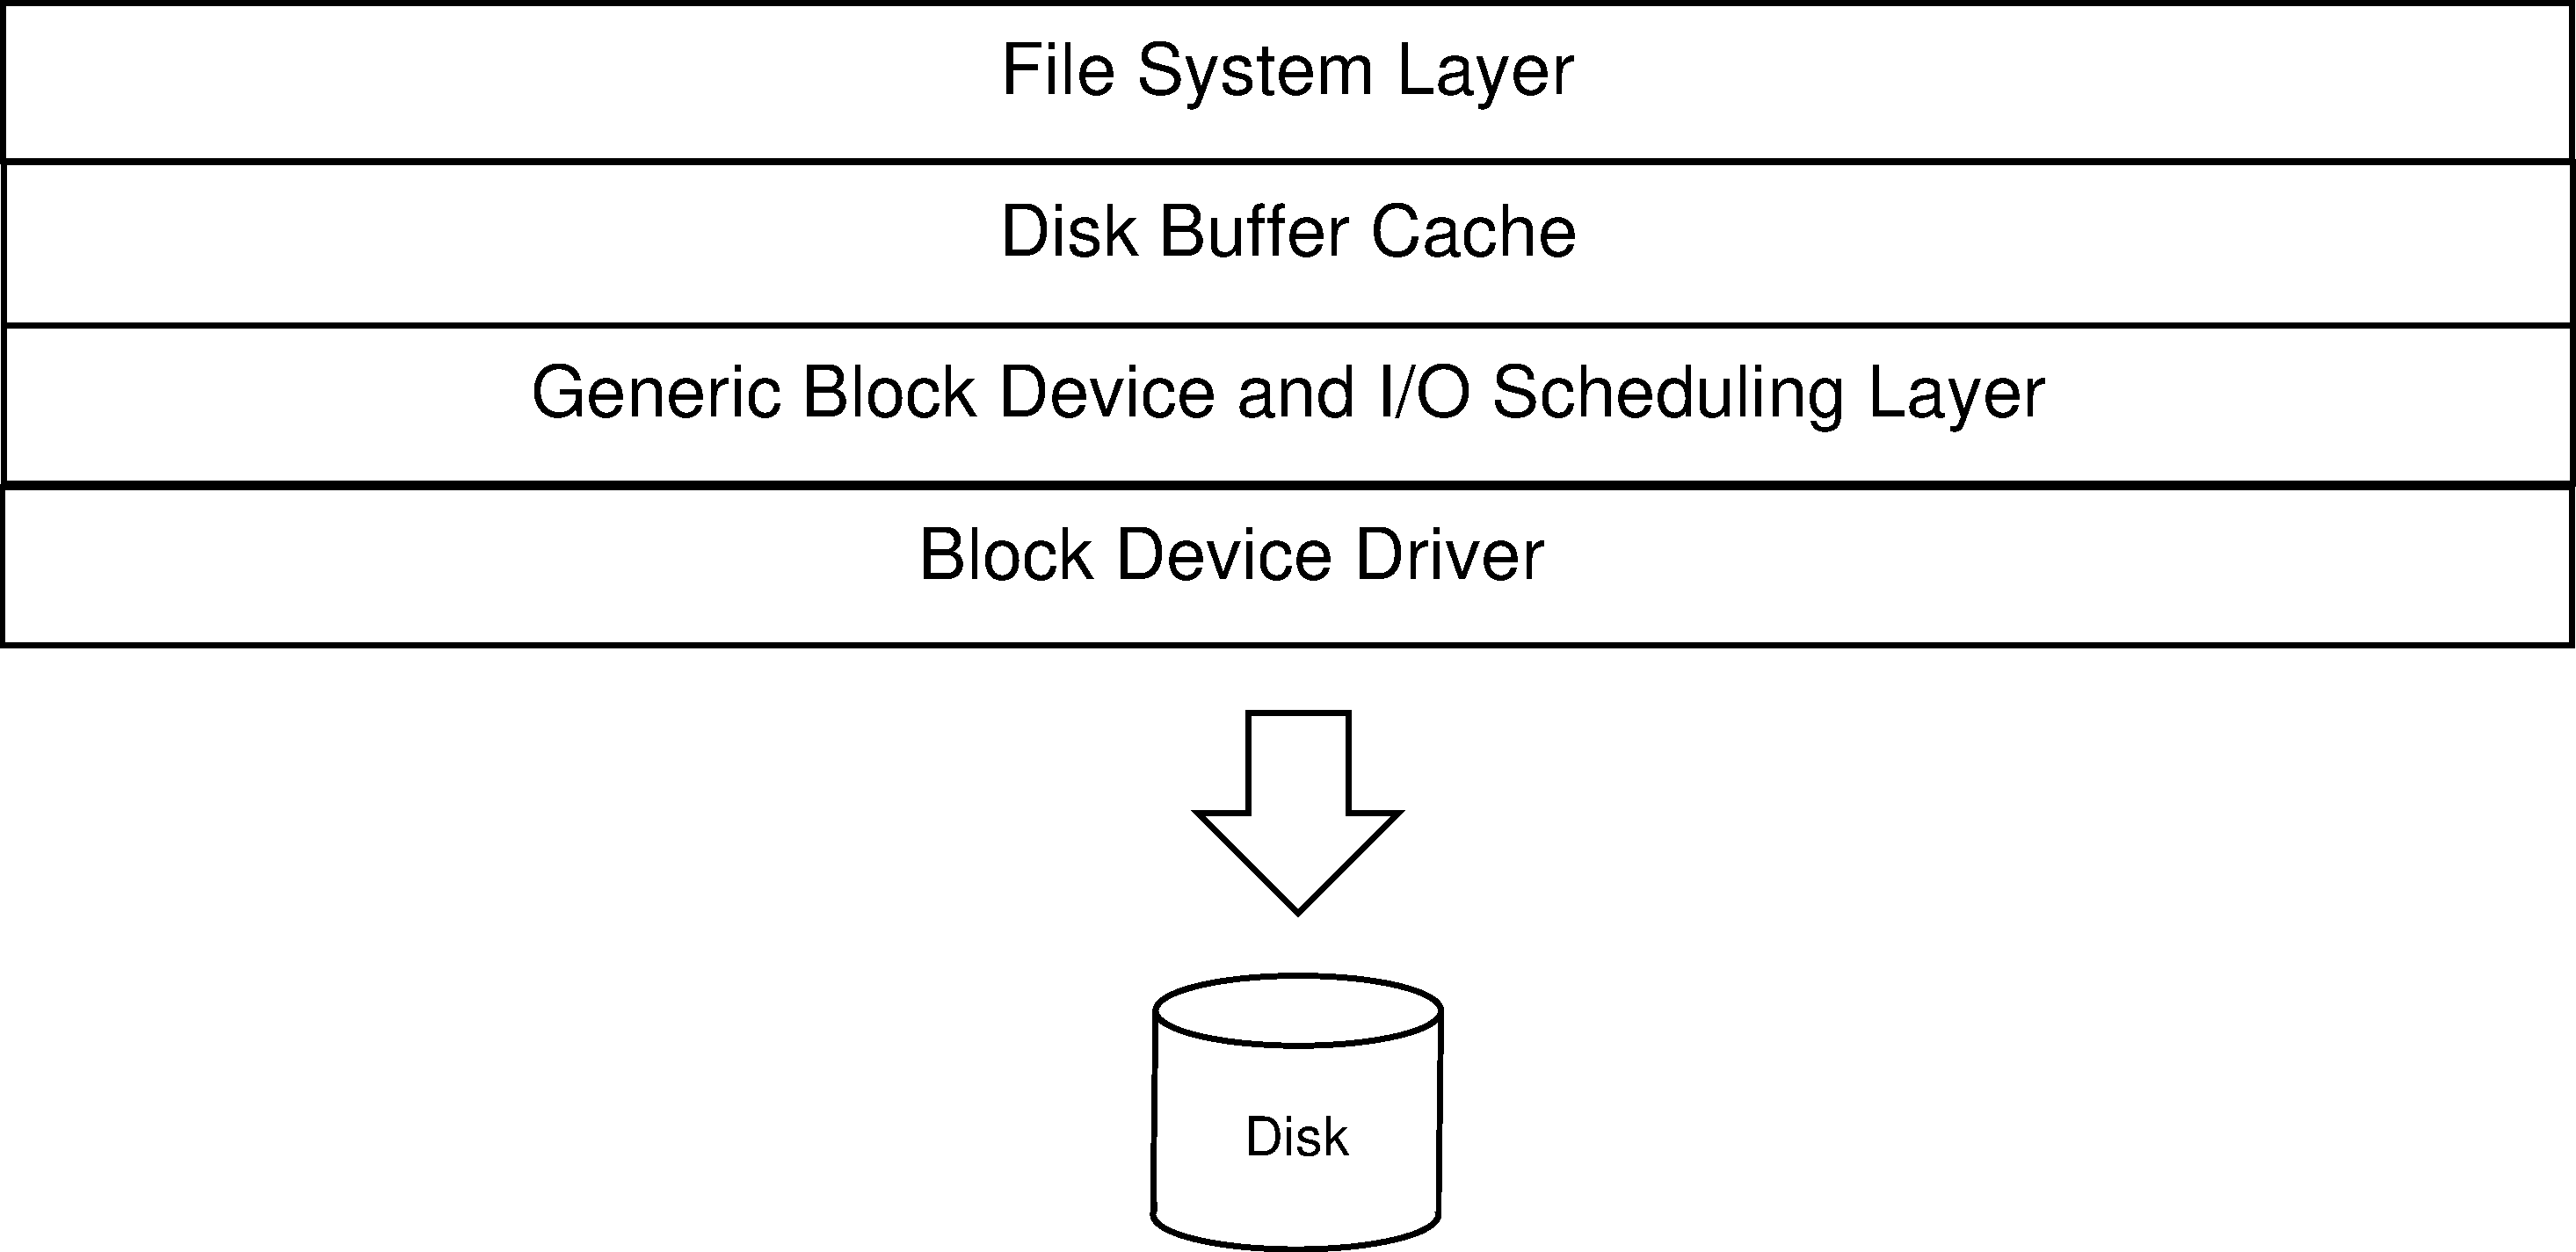
\includegraphics[width=0.7\columnwidth]{figs/block-fs-disk}}
\caption{File system architecture}
\label{fig:block-fs}
\end{figure}

Operating systems have traditionally provided support for persistent
storage through file systems. Files are read (or updated) by making
system calls which copy a region of memory from (or to) the
device. Introduced in the Multics input/output
system~\cite{Feiertag72}, the file interface is widely established and
is also used to access other devices like network cards in UNIX based
operating systems. The file system architecture in Linux is shown in
Figure~\ref{fig:block-fs}. Consider a write request for updating a
particular region of a file. First, the request passes through the
file system layer where changes to file system data structures like the
inode map are made. Then the updated pages are buffered in the disk
buffer cache. Pages marked as dirty in the disk buffer cache are then
periodically flushed to the block device layer, which is used to schedule
I/O operations for the hardware. The block device layer also supports
buffered I/O where a block of data can be read, modified and then
written back to the device. With the advent of non-volatile
byte-addressable memory, we believe that the overhead imposed by these
layers will be significant compared to the access latency for NVBM.

In order to measure the overhead at each layer, we perform an experiment where
a region of memory is updated in blocks of different sizes. Since NVBM is not
yet commercially available, we perform the experiments on DRAM, which has been
shown to be a good indicator of NVBM performance~\cite{Condit09}. All our
experiments were performed on a server with two Intel Xeon Quad-Core 2.67~GHz
(X5550) processors and 48~GB of 1333~MHz DDR3-RAM.  Each processor has 128~KB
L1, 256~KB L2, and 8~MB L3 caches. We used the Ubuntu~10.04 Linux distribution
and the 2.6.32-24 64-bit kernel.

\section{Direct Mapped Access}
For measuring the overhead at each layer, we use a direct mapped
experiment, where a region of memory is mapped into the application
and updates are performed directly on it, as a baseline. In the
baseline experiment there are no system calls invoked during the
updates. Updates of different sizes are performed using
\texttt{memcpy} and in order to ensure that there is no overhead due
to page faults, we first write to the entire region before beginning
the updates. The memory bandwidth obtained for different update sizes
is shown in Figure~\ref{fig:serial-large-block} and
Figure~\ref{fig:serial-small-block}. The memory bandwidth for direct
mapped access increases as the size of the updates increase from 1GB/s
for 2 byte updates to 9.1 GB/s for 128 byte updates. We believe this
is related to the number of bytes that can be transferred using one
SSE instruction.

\begin{figure}[t]
\begin{minipage}[b]{0.47\linewidth}
\centerline{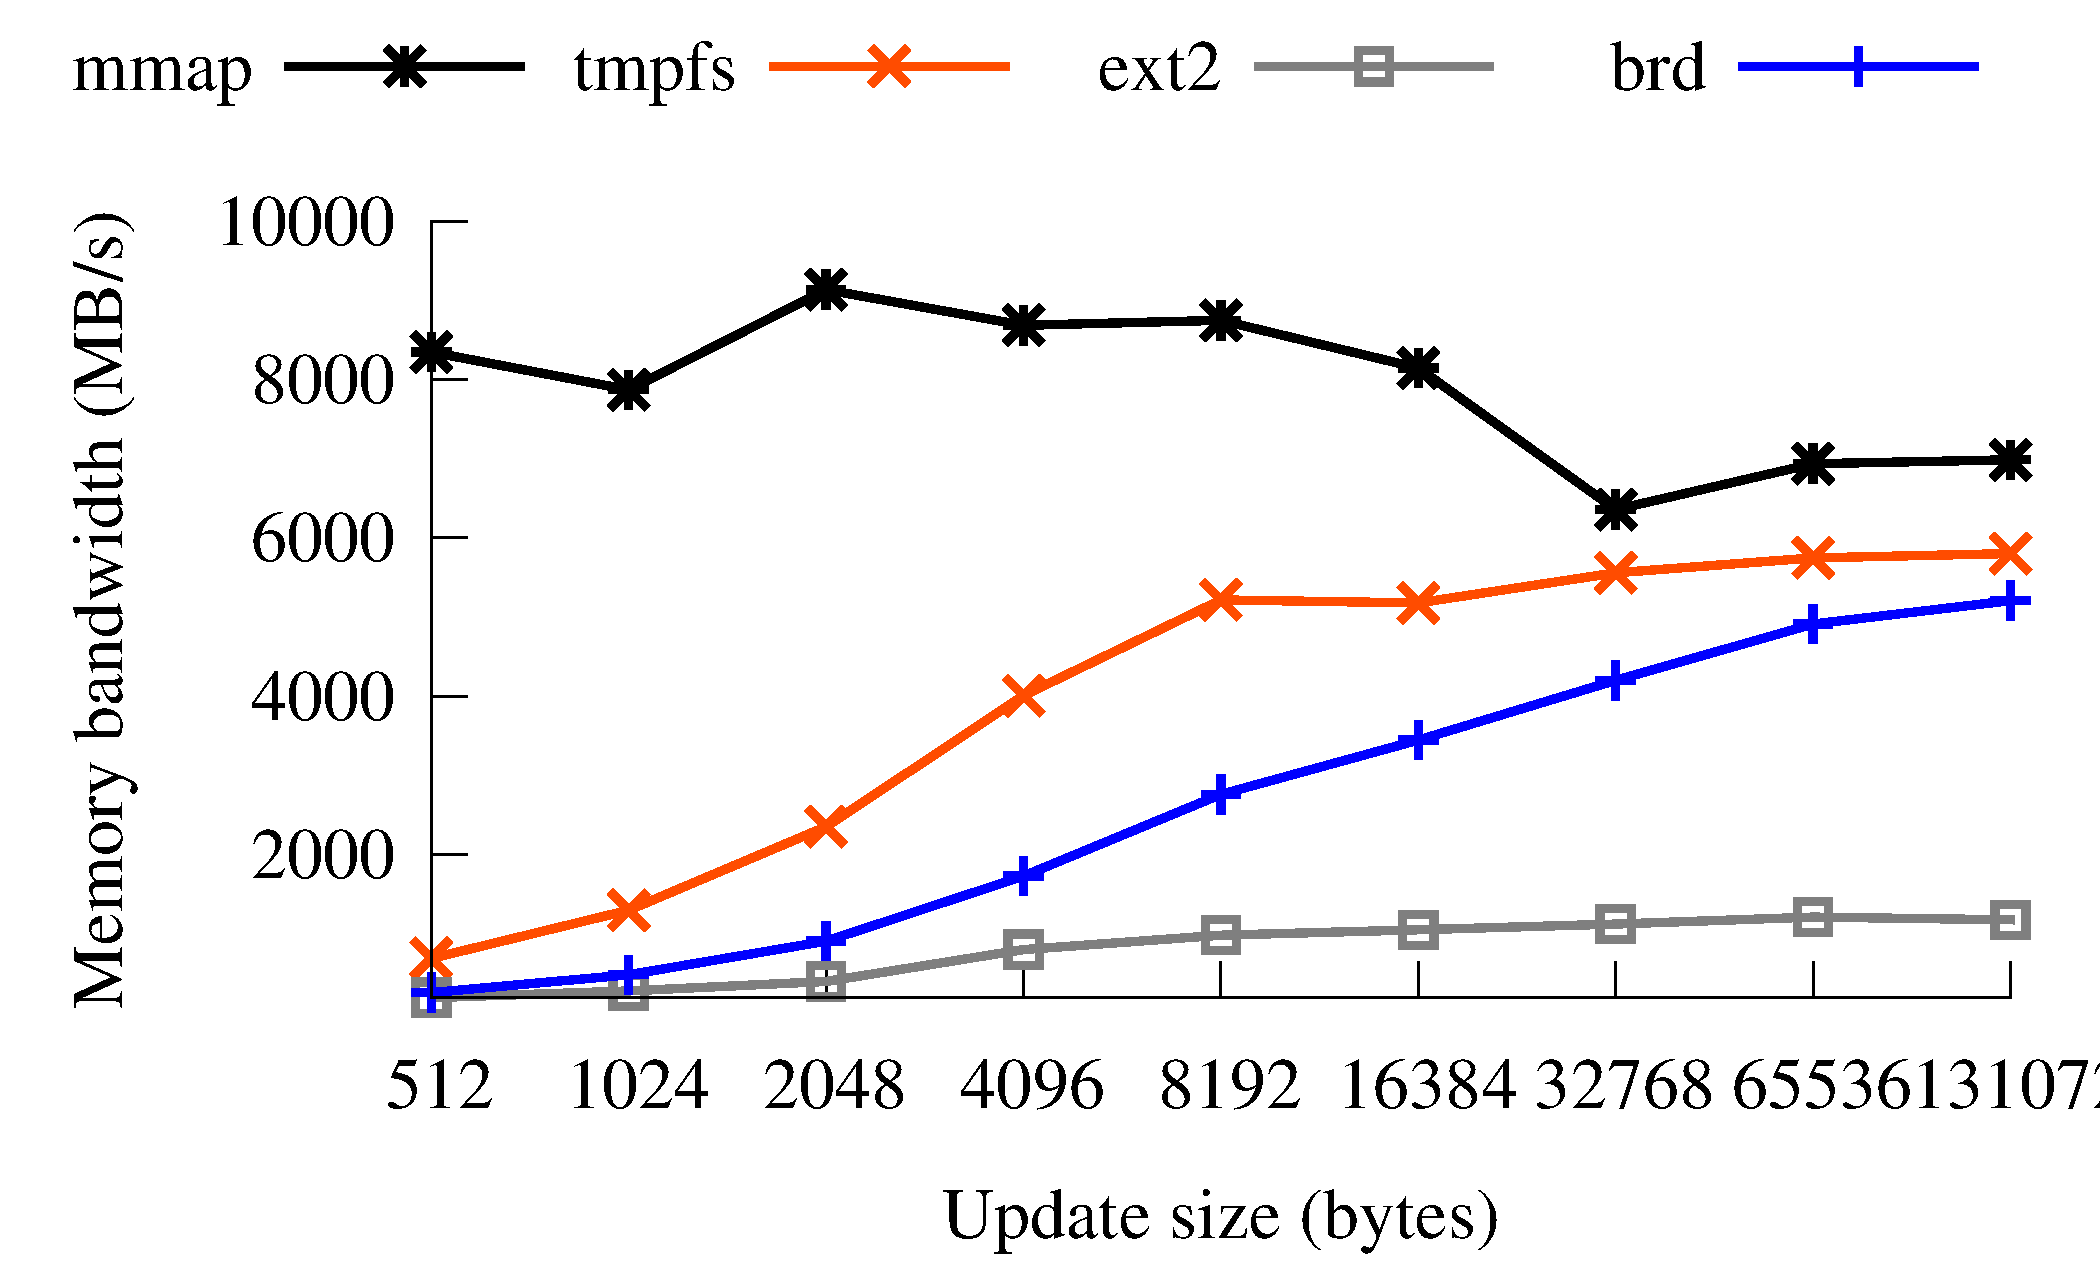
\includegraphics[width=\columnwidth]{figs/block-fs-large}}
\caption[Block device and File system overhead for large updates]
        {Block device and File system overhead for large updates. Note
         the linear scale on the y-axis}
\label{fig:serial-large-block}
\end{minipage}
\hspace{0.04\linewidth}
\begin{minipage}[b]{0.47\linewidth}
\centerline{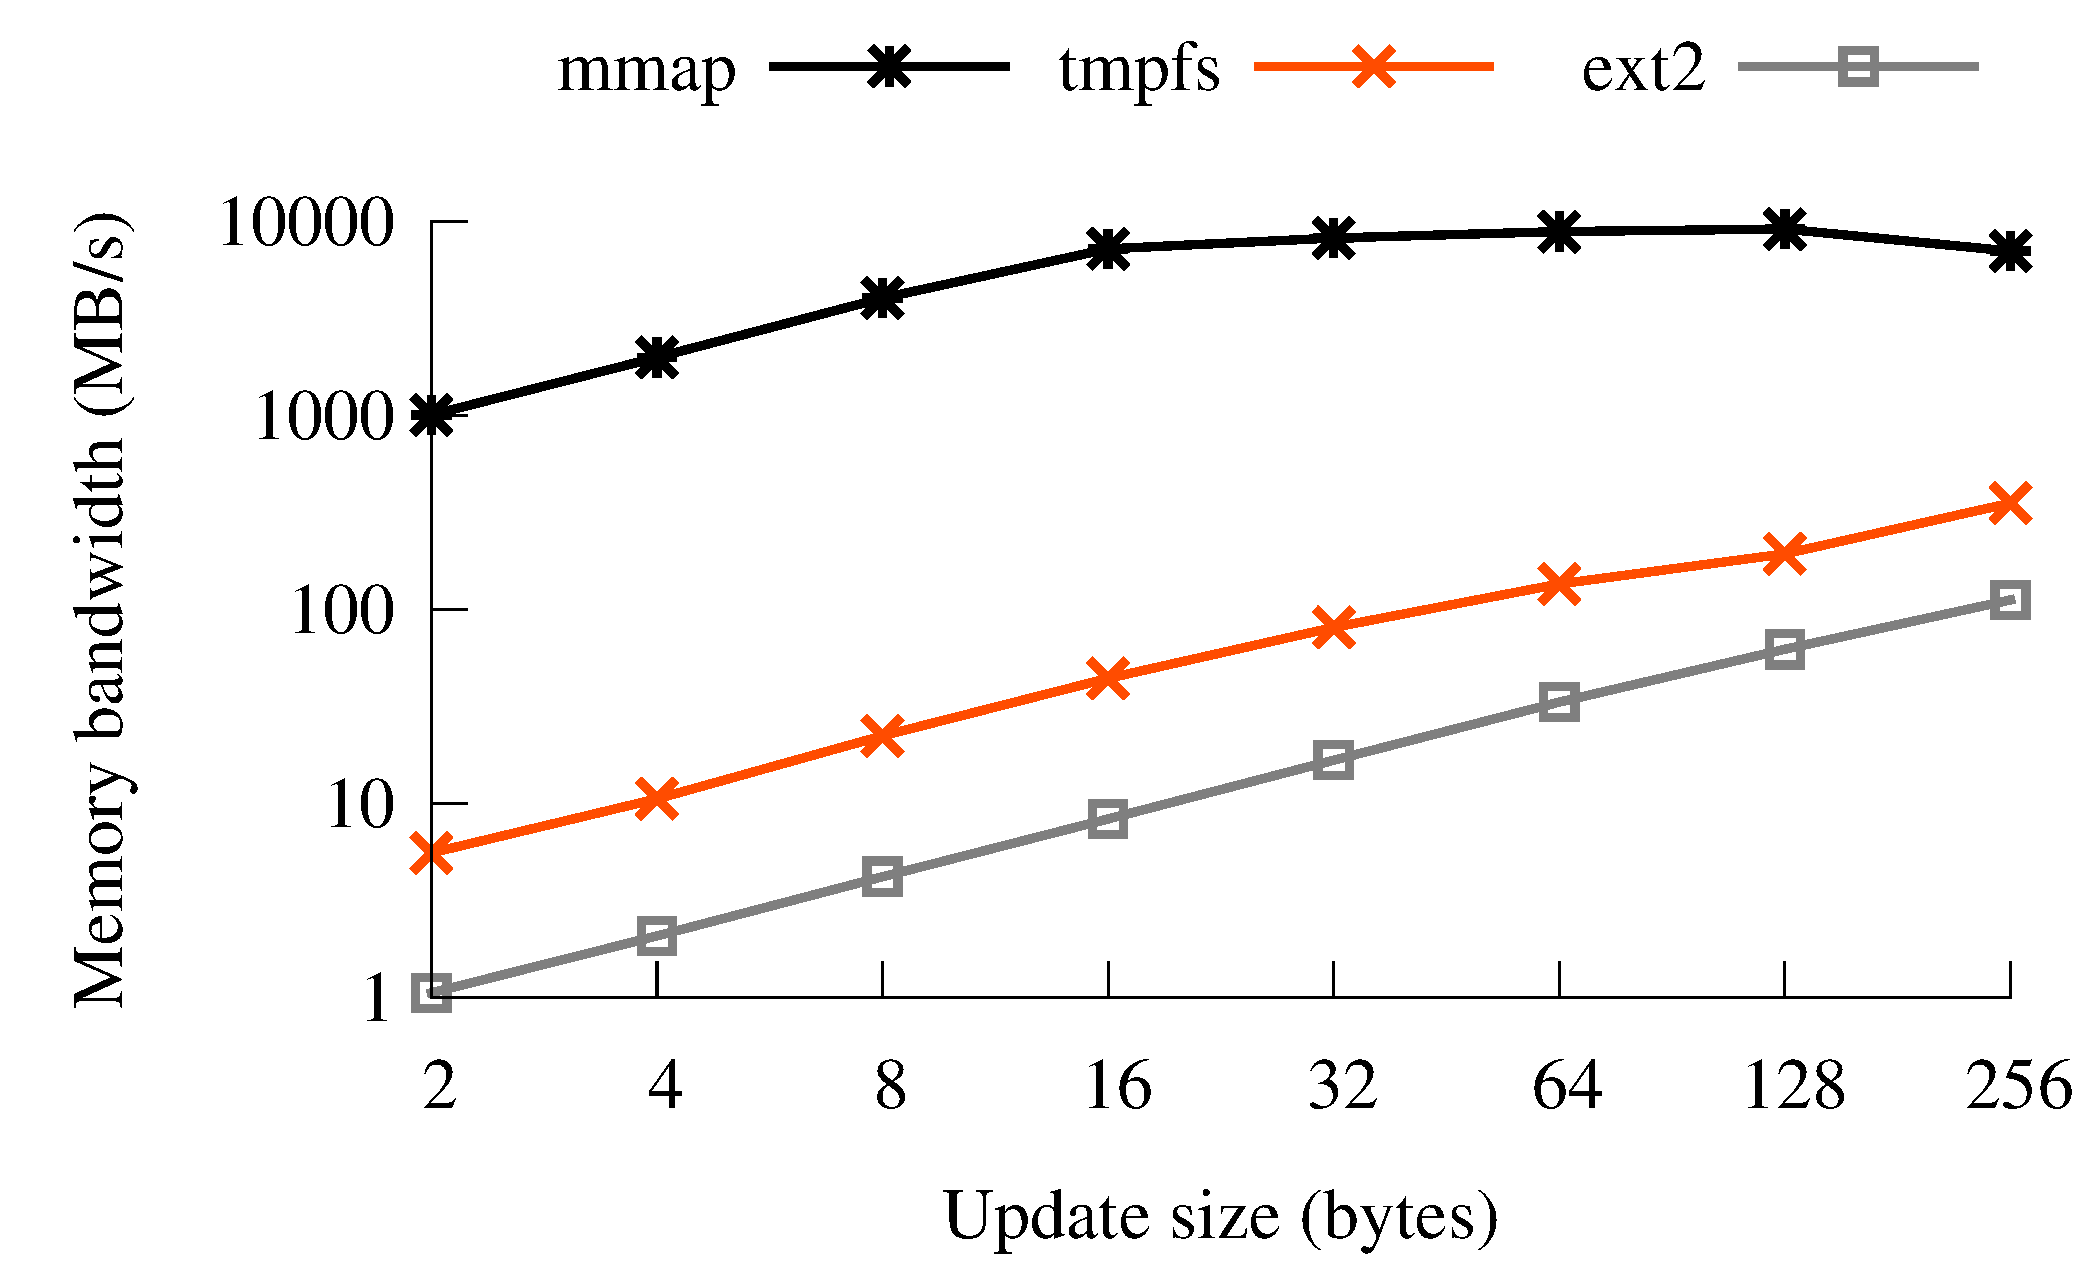
\includegraphics[width=\columnwidth]{figs/block-fs-small}}
\caption[Block device and File system overhead for small updates.]
        {Block device and File system overhead for small updates.  Note
        the log scale on the y-axis.}
\label{fig:serial-small-block}
\end{minipage}
%\vspace{-0.15in}
\end{figure}

\section{Block Device Layer}
To measure the overhead imposed by the block device layer, we measure
the performance of using the Block RAM device (BRD)~\cite{brd-linux}
to perform serial writes to a region of memory. The Block RAM device
in Linux exposes main memory as a block device and we perform updates
using write calls directly to the device, without mounting any
file system on it. Also in order to ensure that the writes are not
cached at the disk buffer cache, we open the device using the
O\_DIRECT flag. In this case, updates to the file are directly flushed
to the block device. The results presented in
Figure~\ref{fig:serial-large-block} show that as the block size is
varied between 512 bytes and 128KB, the overhead of using the block
device layer varies between $32$x and $1.3$x in terms of memory
bandwidth. (We were unable to perform updates smaller than 512 bytes
using O\_DIRECT as direct updates need to be multiples of the disk
sector size. This is another indication that the block device layer is
tuned for disks.)

\section{File Systems}
We consider two different configurations to demonstrate the overhead
of using a file system and correspondingly the file interface. First,
we mount ext2 on BRD and measure the time required to perform serial
writes to a file. The results shown in
Figure~\ref{fig:serial-small-block} show that mounting ext2 on BRD
performs worse than writing directly to the device. This is due to the
additional overhead of the file system layer which is combined with
that of the block device interface.

We also considered \texttt{tmpfs}~\cite{tmpfs} an in-memory file
system in Linux, where the data is stored in the page cache. As a
result, there is no block device overhead in this case and we can
measure the overhead of the file system layer. The results shown in
Figure~\ref{fig:serial-small-block} show that for smaller 64B block sizes,
direct mapped access is $65$ times faster than using
\texttt{tmpfs}. However as the block size is increased to 4K, we find
that the performance converges to within 83\% of direct mapped
access.

\begin{figure}[t!]
\begin{minipage}[b]{0.45\linewidth}
\centerline{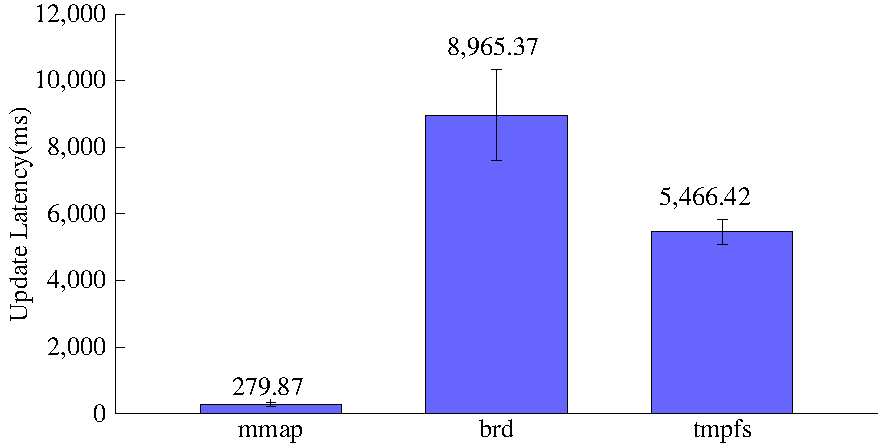
\includegraphics[width=\columnwidth]{figs/flush-fs}}
\caption{Latency for cache line sized update and flush}
\label{fig:random-update}
\end{minipage}
\hspace{0.04\linewidth}
\begin{minipage}[b]{0.45\linewidth}
\begin{center}
\begin{tabular}{cc}
\toprule
System & No. of function calls \\
\midrule
tmpfs & 64 \\
Block RAM Device (BRD) & 136 \\
ext2 on BRD  & 192 \\
\bottomrule
\end{tabular}
\captionof{table}{Number of kernel functions invoked in one \texttt{sys\_write} system call}
\label{tab:syscall}
\end{center}
\end{minipage}
\end{figure}

\section{Flush Overhead}
Since NVBM will be available through DIMM slots, we can flush cache line
sized updates to the device. However the block device and the
file system layer can only flush updates which are equal to the page
size (4KB in Linux). We performed an experiment to measure the
overhead due to this limitation. In this experiment, we create a file
of a fixed size and seek to a random location in the file. We then
perform a cache line sized update and flush the update to NVBM using the
\texttt{fsync} call. The Block RAM device and \texttt{tmpfs} layers were
modified to invoke the \texttt{clflush} instruction for a sync
operation. We compare the time taken against performing
\texttt{clflush} from a userspace application. The results of this
experiment are shown in Figure~\ref{fig:random-update}. The time taken
to update and flush a cache line is around 280ns from the userspace
application. When compared to direct mapped access, the latency
of using \texttt{tmpfs} and the Block RAM device is greater by $19.5$x
and $32$x respectively. 
% There are some possible additional issues like the granularity of
% transactions and coordination at  a block level is inefficient -
% False sharing. Reading large chunks of file systems into memory causes
% large number of cache invalidations and cache use overhead - NVBM would
% allow finer grain access control (cf files or databases), far less false
% sharing for shared data, and far less cache invalidations for
% shared data, and far less cache invalidations for applications that are
% only doing partial updates on files

\section{System Call Overhead}
In addition to measuring the memory bandwidth and latencies, we profiled the
kernel functions invoked for every system call using LTTng~\cite{lttng}, a
Linux-kernel tracing tool. The number of function calls invoked for a single
\texttt{sys\_write} system call for \texttt{tmpfs}, BRD and ext2 on BRD is
shown in Table~\ref{tab:syscall}. While the system call implementations have
been optimized over the years, their performance will always be slower than
performing no system calls at all.  Hence, providing direct mapped access to
NVBM removes the operating system from the critical path and overcomes any
overheads for performing reads and writes.  However, the OS will play in
important role in providing isolation for directly mapped pages and
we discuss issues related to safety in Chapter~\ref{sec:conclusion}.
